\documentclass[11pt,a4paper]{article}
\usepackage[margin=2.5cm]{geometry}
\usepackage[utf8]{inputenc}
\usepackage[T1]{fontenc}
\usepackage{hyperref}
\renewcommand{\familydefault}{\sfdefault}
\usepackage{helvet}
\pagestyle{empty}
\usepackage[kerning=true]{microtype}
\usepackage{parskip}
\usepackage{sansmath}
\usepackage[font={small, bf}]{caption}
\usepackage[font={small}]{subcaption}
\usepackage{graphicx}
\usepackage{multicol}
\setlength{\abovecaptionskip}{0pt}
\setlength{\floatsep}{10pt}
\setlength{\textfloatsep}{0pt}
\setlength{\intextsep}{0pt}
\setlength{\belowcaptionskip}{0pt}
\setlength{\parindent}{5ex}
\setlength{\parskip}{0pt}
% Feel free to use additional packages for glosses, figures, whatnot.

% The next bit is for reserving sufficient space for authors,
% affiliations, and e-mail address.  No need to change for initial
% anonymous version.  For the final version, replace the
% \toggletrue{anonymous} with \togglefalse{anonymous} to de-anonymize.
\usepackage{etoolbox}
\newtoggle{anonymous}
\togglefalse{anonymous}

\renewcommand{\title}[1]{\textbf{#1}\\}
\newcommand{\authors}[1]{\iftoggle{anonymous}{\phantom{#1}}{#1}\\}
\newcommand{\email}[1]{\iftoggle{anonymous}{\phantom{#1}}{#1}}

\begin{document}

% First page:

% Insert title, authors, affiliations, and e-mail address in the next three lines:

\title{Thick feedback facilitates referential coordination in larger groups}
\authors{Veronica Boyce\textsuperscript{1}, Robert D.  Hawkins\textsuperscript{2}, Noah D. Goodman\textsuperscript{1}, Michael C. Frank\textsuperscript{1}} 
\email{vboyce@stanford.edu;  \textsuperscript{1}Stanford, \textsuperscript{2}Princeton}
\newline
%

% Intro
%TODO citations
Shared referring expressions are necessary for efficient communication. When there are not conventional names for objects, interlocutors create spontaneous ad-hoc expressions. The formation and adoption of these new referring expressions is well-studied in dyadic iterated reference games (Clark \& Wilkes-Gibbs 1986). Over repetition, a few key phenomena emerge: listeners have high and increasing selection accuracy while speakers' referring expressions shorten as shared conceptualizations result in partner-specific nicknames. These patterns are also found in small groups where a speaker addresses up to 5 listeners at once (Yoon \& Brown Schmidt 2019, Boyce et al. 2022). Here we begin to address what properties of the communication channel support these phenomena and whether they differ by group size.

\textbf{Methods:} We conducted a 2x2 experiment crossing group size (2 or 6 players, 6 matches the largest groups in Boyce et al. 2022) with communication channel width. In \textbf{thick} games (maximizing communication and shared knowledge), one  player was the speaker the entire time, the speaker and listeners could  all send chat messages, and all players saw who selected what image and whether it was right. In the \textbf{thin} condition, the speaker role rotated each block, only the speaker could send chat messages while listeners were limited to sending 4 emojis to indicate their level of understanding, and listeners only saw feedback on their own selections.


We recruited English-speaking participants from Prolific to play a real-time communication game implemented in Empirica (Almaatouq et al. 2021). Participants saw 12 tangram figures, the speaker described the target to the listeners using the chat box, and listeners clicked on their selection (Fig 1). Speakers and listeners received feedback at the end of each trial. After all 12 tangrams were described, the process repeated for a total of 6 blocks (72 referential trials). We ran roughly 40 games in each of the 4 conditions for a total of 623 participants (160K words). 

% Results

\textbf{Results:} In line with prior work, we found increasing listener accuracy and decreasing utterance lengths over the course of the game (Figs 2A and B). Speakers used fewer words in 2 player games compared to 6 player games independent of block. Both group size and channel width affected listener accuracy: 2 person groups and thick channels had higher accuracies. 

We embedded the speaker's utterances using S-BERT (Reimers \& Gurevych 2020) which mapped the speaker's language on each trial to a vector in a high-dimensional semantic space. %We then used cosine similarity between pairs of vectors as a proxy for similarity between pairs of utterances. 
To look for the emergence of group-specific descriptions, we took cosine similarities between embeddings of descriptions of the same tangram in the same block in different games. If groups developed partner-specific nicknames, similarity would decrease over time. We found decreasing similarity in 2 player games and 6 player thick games (Fig 2C). The 6 player thin games showed a much flatter pattern, suggesting less differentiation between games. 

To measure within-group convergence to a shared convention, we treated final block utterances as the ``convention'' and measured the cosine similarity of earlier utterances in the same game for the same tangram to this final convention. Convergence to a convention would mean increasing cosine similarity across blocks. Similarity increased across all conditions; however, thick games increased faster and more strongly, indicating faster convergence to nicknames, while 6-player thin games increased only a little (Fig 2D). 

\textbf{Conclusion:} We examined how group size and communication channel width jointly influenced participants performance in an iterated reference game. Participants in all conditions showed reduced utterances and increased accuracy over blocks. However, the 6-player thin games did not show convergence to the shared, partner-specific conventions seen in other conditions. This suggests that thick channels can rescue communication and hold larger groups together, while dyads form conventions even with constrained communication. However, channel thickness was a composite of greater feedback, listener backchannel, and speaker consistency; determining which aspects are key to larger group success is a future direction.  
\newpage

\begin{figure}
	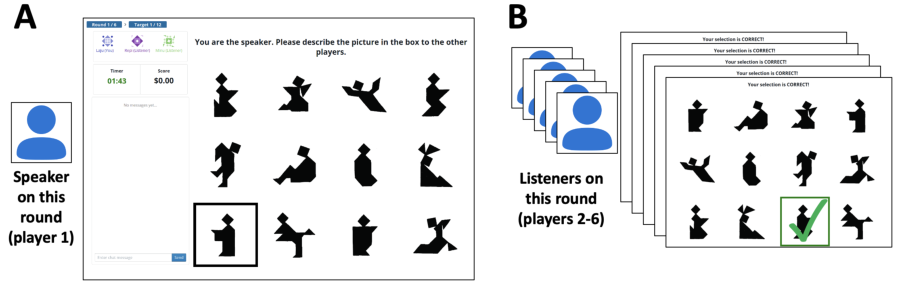
\includegraphics[width=\textwidth]{../images/interface-1.pdf}
	\caption{Schematic of player interface}
\end{figure}

\begin{figure}
	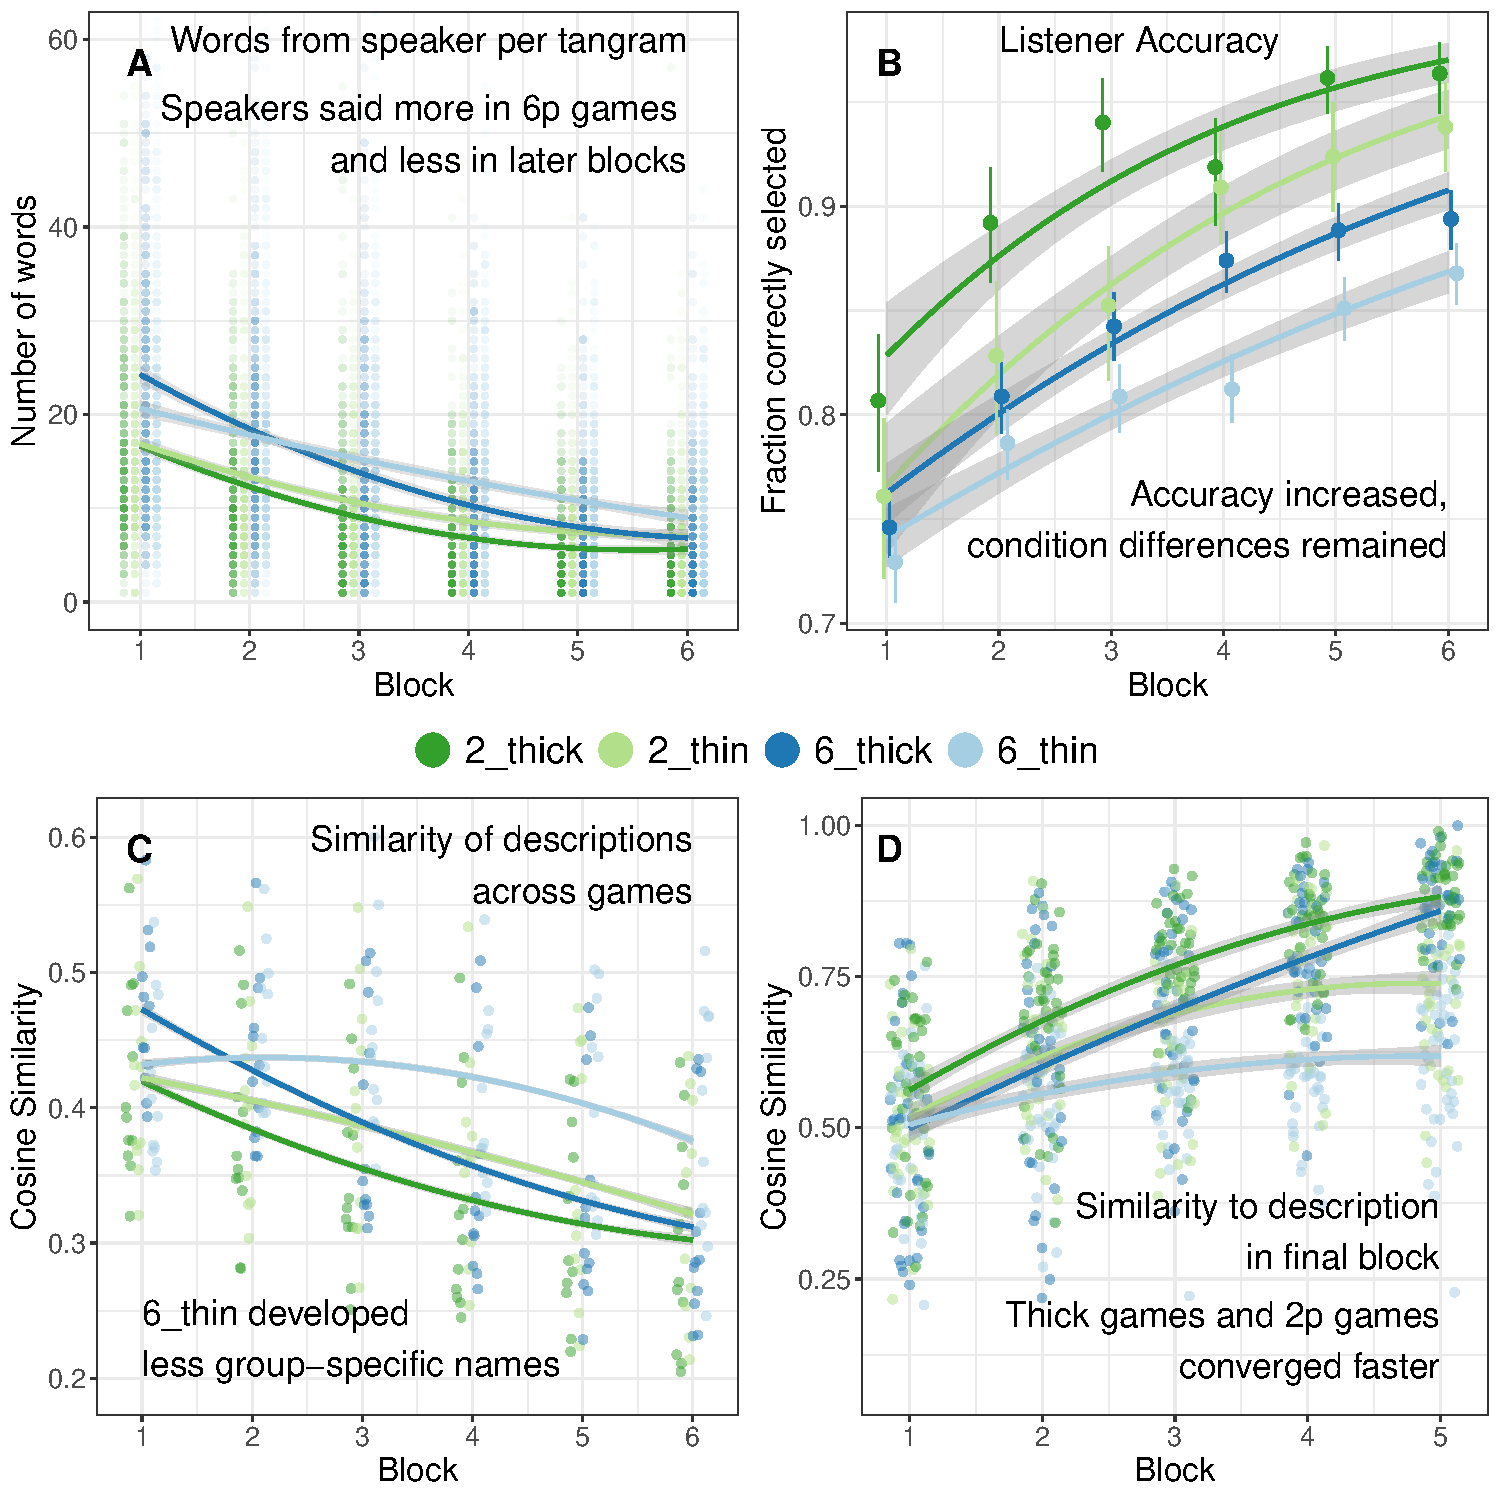
\includegraphics[width=\textwidth]{../images/CAMP1.pdf}
	\caption{Results by condition}
\end{figure}

\begin{figure}\textbf{References:}  Almaatouq, Becker, Houghton, Paton, Watts \& Whiting. Behavioral Research Methods 2021. 
$\bullet$ Boyce, Hawkins, Goodman \& Frank. 44th CogSci 2022.
$\bullet$ Clark \& Wilkes-Gibbs. Cognition 1986.
$\bullet$ Reimers \& Gurevych. EMNLP 2020. 
$\bullet$ Yoon \& Brown-Schmidt. Cognitive Science 2019.
  \end{figure}

\end{document}